\chapter {Quick Reference: Component Details}
\section{BJT BF194/195}
\label{BF194/195}
BF194/195 is a high frequency transistor. From its datasheet 

Type Designator: BF194/BF195

Material of transistor: Si

Polarity: NPN

Maximum collector power dissipation ($Pc$), W: 0.25

Maximum collector-base voltage |$V_{cb}$|, V: 30

Maximum collector-emitter voltage |$V_{ce}$|, V: 20

Maximum emitter-base voltage |$V_{eb}$|, V: 5

Maximum collector current |$I_{c max}$|, mA: 30

Forward current transfer ratio (hFE), min: 67

\textcolor{red}{TODO: Pinout diagram to be added}
\section{BJT BC107}
\label{BC107}
Type Designator: BC107

Material of transistor: Si

Polarity: NPN

Maximum collector power dissipation ($P_c$), W: 0.3

Maximum collector-base voltage |$V_{cb}$|, V: 50

Maximum collector-emitter voltage |$V_{ce}$|, V: 45

Maximum emitter-base voltage |$V_{eb}$|, V: 6

Maximum collector current |$I_{cmax}$|, A: 0.1

Forward current transfer ratio ($h_{FE}$), min: 110

Package of BC107 transistor: TO18
\textcolor{red}{TODO: add schematic diagram and photo of BC107}

\section{Intermediate Frequency Transformer}
\label{IFT}
IFT act as parallel resonant circuits whose resonating frequency is around 455 kHz. This frequecy is adjustable by a factor of  \textcolor{red}{FIXME} plusorminus 10\%. IFT has a tappedd primary winding and a secondary winding. Primary winding has a capacitor connected in parallel internally. Its inductor value is $L_eq=450\ mu H$ and capacitance $C=270\ pF$. 
\\Its resonant frequency is thus $f=\frac{2\pi}{\sqrt{L_{eq}C}}\approx 455 kHz$.

\textcolor{red}{TODO: add schematic diagram and photo of IFT}
\section{AD 633 - Multiplier IC}
Analog multipliers are complex arrangements of Opamps and other circuit elements in the form of IC. It can be used for different applications like multiplication, division, squarer, modulator, demodulator, filter etc. There are two inputs X and Y to which the signals to be multiplied are given.
\begin{figure}[h]
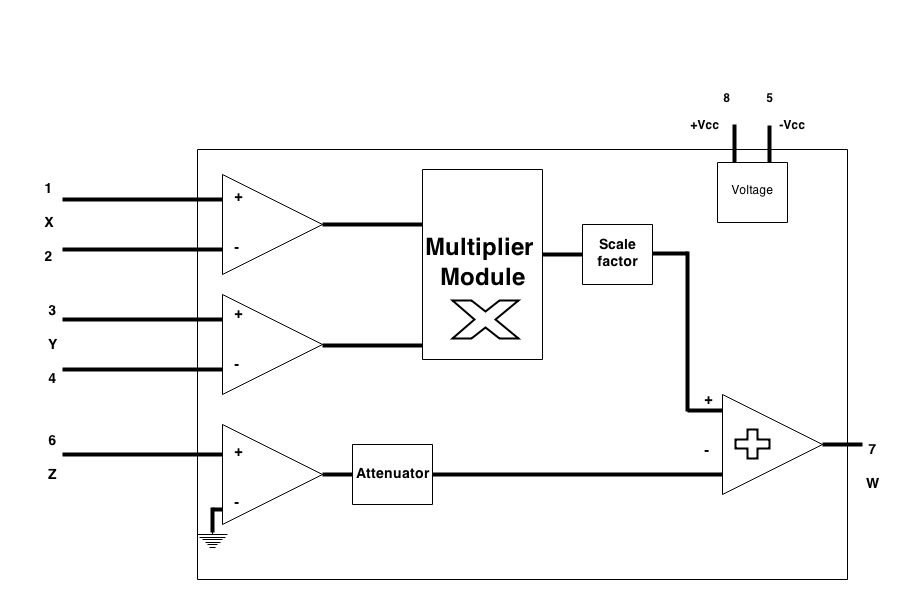
\includegraphics[width=10cm, height=7cm]{ad633.png}
\caption{Functional Block Diagram for AD633 multiplier IC}
\end{figure}